%%
%% Capítulo 1: Introdução
%%

\mychapter{Introdução}
\label{Cap:Introducao}
% Dicas para o trabalho
% [A revisar] [Revisado]{Adicionado com outras palavras}{Fazer uma ou duas perguntas relacionadas ao trabalho que serão respondidas no decorrer do mesmo.
% O objeto do projeto é tornar o registro de dados sobre a vacinação contra a COVID-19 mais fácil e rápido para os profissionais de saúde, de forma que possam se concentrar em outras atividades. Esse registro é feito manualmente e em papel, o que pode gerar erros e atrasos no processo de cadastro. O objetivo do projeto é criar um sistema que organize os dados e envio-os por meio de planilhas que poderão ser enviadas ao sistema único de saúde.}

% [A fazer] [Revisado]{Adicionado com outras palavras}{Escrever por que essa solução deve ser usada e qual o problema ele resolve.}

% [As informações de Titita][Revisado]{Não adicionado}{Existem dois sistemas para informação das vacinações do município: esus pec e o novo sipni.}
%  [Revisado]{Adicionado com outras palavras}{O manual de vacinação
% O velho sipni (sipni web) era usado paras campanhas de vacinação contra influenza e poliomelite. Agora todas as campanhas são feitas no novo sipni. Nesse ano de 2022 já foram feitas campanhas contra sarampo, polio e influenza.}

% Cada campanha tem um manual técnico/operacional.}


\section{Contextualização}
\label{cap1:Sec:Contextualizacao}
Em 2019 surgiu o vírus SARS-Cov-2 (Síndrome Respiratória Aguda Grave), responsável por causar a maior pandemia já registrada na história, chamada Covid-19. Desde então, uma grande mobilização em todos os países começou visando a criação de uma vacina contra a doença causada pelo vírus e a consequente corrida para a sua produção em massa. De acordo com a Organização Mundial da Saúde (OMS), no início de 2021 existiam 236 vacinas candidatas em fases pré-clínicas ou fase clínica \cite{ministerio2022plano}.


No Brasil, a vacinação contra a COVID-19 começou em 18 de janeiro de 2021, com a vacina Coronavac, produzida pelo Instituto Butantan em parceria com a farmacêutica chinesa Sinovac. A vacinação foi realizada em etapas, à medida em que as vacinas eram fabricadas e priorizando os grupos de maior risco de contaminação e de complicações da doença: profissionais da saúde, idosos, pessoas com comorbidade, pessoas com deficiência e população indígena. A vacinação foi feita em todo o país e com a utilização de um plano nacional, mas cada estado e município teve sua própria estratégia para a vacinação, em geral, pautada nesse plano \cite{ministerio2022plano}.


Independente da estratégia de vacinação de cada estado e em decorrência da necessidade de mapear com exatidão as pessoas que receberam a vacina, o Ministério da Saúde criou um módulo online (Figura \ref{fig:sipni_login}) para o registro de dados nominais sobre a vacinação, o que inclui dados pessoais d(a) vacinado(a), dose e lote administrados. Esse sistema foi denominado Sistema de Informações do Programa Nacional de Imunizações (Novo SI-PNI) e é usado para o registro de dados sobre as campanhas de vacinação.

\begin{figure}[!ht]
  \centering
  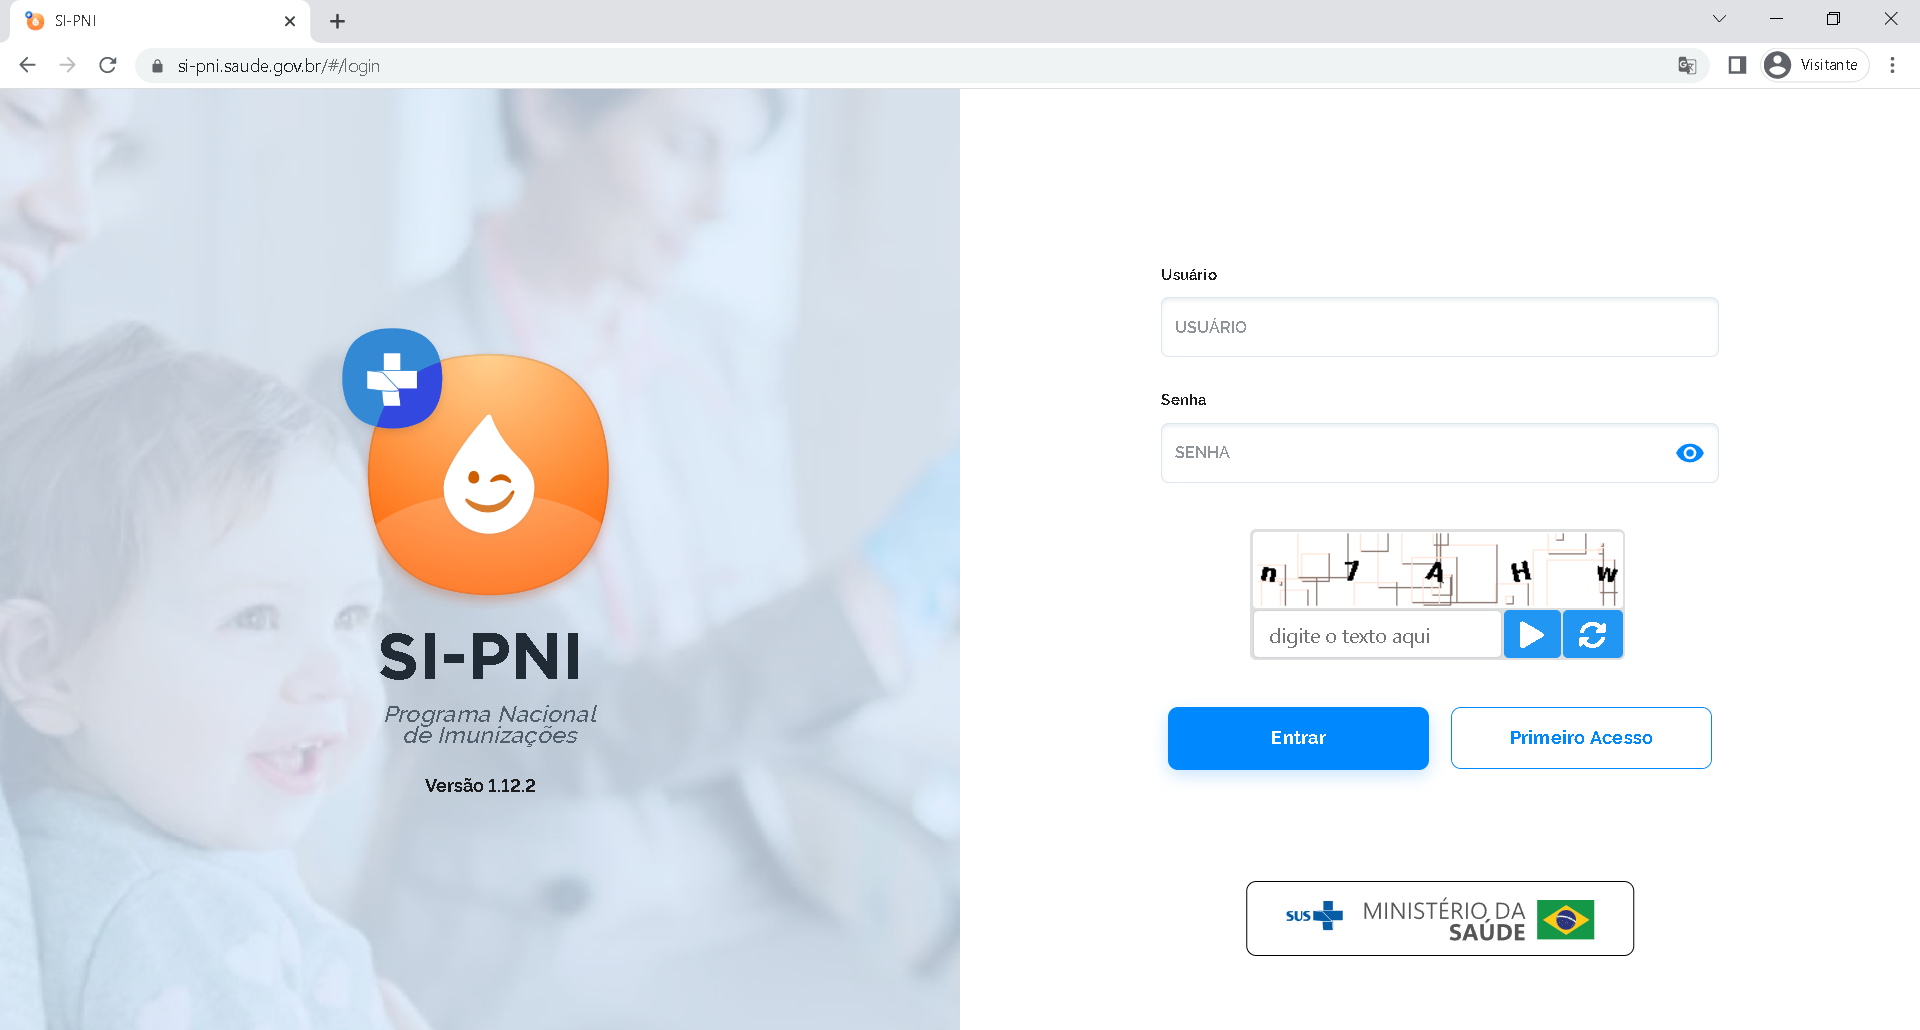
\includegraphics[width=0.8\textwidth]{figuras/cap1/1_1_pagina_login_sipni.png}
  \caption{Tela de login do novo SI-PNI}
  \label{fig:sipni_login}
\end{figure}

\section{Problemática}
\label{cap1:Sec:Problematica}
\subsection{Cenários para vacinação e registro de dados}
\label{cap1:SubSec:CenariosVacinacao}
O registro nominal no paciente que será vacinado pode ser realizado em alguns cenários a depender da infraestrutura do local da vacinação. Onde há conectividade com a internet, esse registro pode ser feito diretamente na plataforma online do SI-PNI (disponível em \url{https://si-pni.saude.gov.br/}) mas, onde não há conectividade ou não há estabilidade na conexão presente no local da vacinação (que pode ser realizado dentro ou fora de um estabelecimento de saúde), o registro deverá ser realizado em formulários impressos com os campos apresentados na seção \ref{cap1:Sec:Contextualizacao} e, posteriormente, redigidos no sistema online \cite{ministerio2022plano}. Os campos mínimos para o formulário são apresentados abaixo e foram retirados do Plano Nacional de Operacionalização da Vacinação contra a Covid-19 \cite{ministerio2022plano}:

\begin{itemize}
  \item CNES (Cadastro Nacional de Estabelecimentos de Saúde) do estabelecimento de saúde
  \item CPF (Cadastro de Pessoa Física)/CNS (Cartão Nacional de Saúde) do vacinado
  \item Data de nascimento
  \item Nome da mãe
  \item Sexo
  \item Grupo prioritário
  \item Data da vacinação
  \item Nome da vacina/fabricante
  \item Tipo de dose
  \item Lote/validade da vacina
\end{itemize}

Um exemplar desse formulário pode ser encontrado no portal do e-SUS APS e está disponível em \url{http://189.28.128.100/dab/docs/portaldab/documentos/esus/ficha_vacinacao_COVID-19.pdf}.

Existem alguma opções de preenchimento desses dados \cite{roteiro2021sipni}:
\begin{enumerate}[label=\textbf{\roman*}]
  \item Registro individual de vacina, onde o operador do sistema pode pesquisar o paciente por CPF ou número do CNS e preencher os dados da vacinação;
  \item Registro em lote manual, no qual o operador preenche os dados de vários pacientes de uma só vez antes de realizar o salvamento no sistema;
  \item Registro em lote por arquivo, no qual o operador realiza o upload de um arquivo com os dados dos pacientes a serem vacinados.
\end{enumerate}

Nesse último caso, quando o conjunto de informações possui vacinações realizadas em dias diferentes ou doses diferentes, estes dados devem ser colocados em arquivos separados para cada dia e dose. Além disso, a planilha recebida pelo sistema deve seguir um padrão pré-estabelecido de quais valores deverão ser adicionados e em quais colunas \cite{roteiro2021sipni}. Abaixo, a lista dos campos que devem ser preenchidos no arquivo-modelo fornecido pelo sistema na página de registro em lote:

\begin{itemize}
  \item CPF/CNS do(a) vacinado(a);
  \item Código sequencial do lote;
  \item Sigla da dose (D1, D2 etc...);
  \item CPF/CNS do(a) profissional de saúde que aplicou a vacina;
  \item Data da vacinação;
  \item Grupo de atendimento prioritário;
  \item Condição maternal do(a) vacinado(a);
\end{itemize}


\subsection{Problema}
\label{cap1:SubSec:Problema}

Levando esses cenários em consideração, existem alguns pontos propensos a erro no processo que poderiam ser evitados. Na coleta de dados, pelo fato de utilização de formulários impressos, existe a possibilidade de equívoco na escrita das informações e/ou na digitação das mesmas no momento em que esses dados são repassados para o sistema online.

Ademais, o trabalho dobrado de registro das informações pode acabar gerando um acúmulo de formulários a serem repassados ao sistema e isso, por sua vez, causa um atraso nas análises que podem vir a ocorrer a partir desses dados para traçar estratégias de combate ao vírus, por exemplo. Por fim, a necessidade de um eventual compartilhamento desses dados se torna um trabalho custoso à medida em que os formulários impressos deverão ser copiados, digitalizados ou transcritos para um formato digital.

Entre as opções de preenchimento dos dados na plataforma \textit{online} apresentados acima, a opção mais produtiva é a última, pois permite que o operador apenas transfira o arquivo com os vacinados para o sistema. Portanto, basta tornar possível a geração desses arquivos de forma rápida e sem a necessidade de realizar o preenchimento manual dos dados novamente após a sua coleta. A aplicação Nurse entra nesse contexto de substituição das fichas de vacinação sem que haja a necessidade de conexão com a internet ou com o sistema online diretamente.

% Ficha de vacinação: https://sisaps.saude.gov.br/esus/ ---> https://sisaps.saude.gov.br/esus/#:~:text=Manual%20PEC/CDS-,Fichas%20%2D%20CDS,-Fichas%20vigentes --->  http://189.28.128.100/dab/docs/portaldab/documentos/esus/ficha_vacinacao_COVID-19.pdf


% [A analisar] [Analisado]{Adicionado com outras palavras}{Posso ir me perguntando vários porquês das coisas e colocar aqui para escrever sobre isso.}

% [A analisar] [Analisado]{Não adicionado}{Posso juntar trabalhos relacionados com problema em um mesmo capítulo.}


\section{Objetivos}
\label{cap1:Sec:Objetivos}

O objetivo geral do trabalho é desenvolver a aplicação \textit{mobile} Nurse, que tem como fim facilitar o registro \textit{offline} de dados sobre as vacinações realizadas pelos profissionais da saúde, reduzir a possibilidade de erros de escrita e de perda de dados, além de agilizar a integração desses dados com o sistema nacional de imunizações. Como objetivos específicos, tem-se:
\begin{itemize}
  \item Apresentar o contexto ao qual a aplicação se destina, destacando-se o problema que ela pretende resolver;
  \item Relatar o processo de desenvolvimento da aplicação, desde a sua concepção até a sua implementação;
  \item Apresentar os resultados obtidos com o desenvolvimento da aplicação;
\end{itemize}

\section{Estrutura do Trabalho}
\label{cap1:Sec:EstruturaTrabalho}

O trabalho está estruturado em seções, como descrito a seguir: 


  \begin{enumerate}[label=\textbf{Seção \arabic*}]
    \item \textbf{Introdução}: trata-se desta seção. Aqui são apresentados o problema, os objetivos e estrutura geral do trabalho.
    \item \textbf{Fundamentação Teórica}: são apresentados os principais conceitos relacionados à plataforma e à modelagem do banco de dados utilizados no desenvolvimento da aplicação.
    % \item \textbf{Trabalhos Relacionados}: descreve aplicações que possuem similaridades com a aplicação Nurse em relação à tecnologia utilizada e/ou área de aplicação.
    \item \textbf{Implementação}: os requisitos, casos de uso e arquitetura da aplicação Nurse, assim como o seu desenvolvimento e os pacotes utilizados para isso são apresentados nessa seção.
    \item \textbf{Experimentos e Resultados}: é nessa seção que são apresentados os testes desenvolvidos para avaliar as funcionalidades da aplicação e os seus resultados. Além disso, são apresentados os principais fluxos se uso da aplicação.
    \item \textbf{Conclusão}: seção dedica às considerações finais sobre o trabalho e as perspectivas futuras para novas funcionalidades que poderão vir a ser implementadas.
    \item \textbf{Referências}: apresenta as referências utilizadas no trabalho.
    \item \textbf{Informações Adicionais}: apresenta, em formato de apêndices, informações adicionais que complementam as informações apresentadas em outras seções do trabalho.
  \end{enumerate}



% \begin{table}[htbp]
% \begin{tabularx}{\linewidth}{|p{3cm}|X|l|} \hline
% COLUNA p & COLUNA X & COLUNA l \\ \hline
% Largura fixa (não depende do conteúdo) &
% Expansível &
% Ajustável \\ \hline
% Alinhada no topo &
% Alinhada à esquerda &
% Alinhada à esquerda \\ \hline
% \end{tabularx}
% \\[0.5cm]
% \begin{tabularx}{\linewidth}{|b{3cm}|C|r|} \hline
% COLUNA b & COLUNA C (ver \texttt{comandos.tex}) & COLUNA r \\ \hline
% Largura fixa (não depende do conteúdo) &
% Expandível &
% Ajustável \\ \hline
% Alinhada na base &
% Centralizada &
% Alinhada à direita \\ \hline
% \end{tabularx}
% \caption{Tabelas com colunas de diferentes larguras e alinhamentos}
% \label{Tab:larguracolunas}
% \end{table}